\chapter{Development}
\label{chapter:dev}

On this chapter we will be explaining how the system was implemented, which algorithms are used and why, and what were the challenges during development.

The system was developed in the Unity engine, utilizing the C\# language. The base of the work was started by following the video tutorial found here \cite{taft:2019}, about creating a 2D top-down game in Unity. Here is where some of the foundation for the work was made, like importing the tileset, understanding how to draw a map, basic collision etc.

After this point is where the creation of the PCG system started. To better understand its implementation we will divide it in 7 steps and discuss each one in a different Section of this Chapter, the last Section will cover all of the user inputs that can be defined in the system in order to tweak the map generation. But first, some information that will be useful to understand all the steps from this point forward: 
\begin{itemize}
    \item The generated map will be represented by a global matrix of integers with width \(w_{map}\) and height \(h_{map}\).
    \begin{itemize}
        \item Its important to notice that \(w_{map}\) and \(h_{map}\) are user-defined parameters.
    \end{itemize}
    \item Each individual integer of this matrix will be referred to as a \emph{cell}.
    \item A cell of value \(1\) represents a \emph{wall}, a cell of value \(0\) represents the absence of a \emph{wall}, or a path.
    \item The Figures where the map is shown are created by the use of Unity's Gizmo debugging tool. On these figures, white represents a \emph{path} cell and black represents a \emph{wall} cell.
\end{itemize}

\section{Create a randomly-filled base map}

The first step taken was to have a randomly generated base map to start building upon.

The generation of random or pseudo-random content generation is a part of most PCG techniques. In our case, the importance of the randomness is given by one of the items for what makes a good map, presented on Section \ref{sec:goodmap} of Chapter \ref{chapter:proposal}: "the Generated maps should look different from one another".

The creation of this base map is accomplished by the steps represented here in Algorithm \ref{alg:randomgen}.


\begin{algorithm}[h] 
 \DontPrintSemicolon
 int map[\(w_{map},h_{map}\)]\;
 \SetKwFunction{FillMapRandomly}{FillMapRandomly}
 \SetKwProg{Fn}{Function}{:}{}
 \Fn{\FillMapRandomly{}}{
  \For{all cells in the map}{
   random = randomly generated number between 0 and 100\;
   \eIf{random < fillPercent}{
    map cell = 1\;
   }{
    map cell = 0\;
   }
  }
 }
 \caption{Randomly filling the map}\label{alg:randomgen}
\end{algorithm} 

The variable \(fillPercent\) will determine how much of the map will be populated by \emph{walls} or \emph{paths}, this variable is a user-defined parameter, and different values will generate different maps at the end. Figure \ref{fig:fillper50} shows an example of a base map with \(w_{map} = h_{map} = 50\) and  \(fillPercent = 50\), and Figure \ref{fig:fillper80} shows the same map but with \(fillPercent = 80\).

\begin{figure}[h]
  \centering
  \begin{minipage}[b]{0.4\textwidth}
    \caption{Map with fillPercent = 50.}
    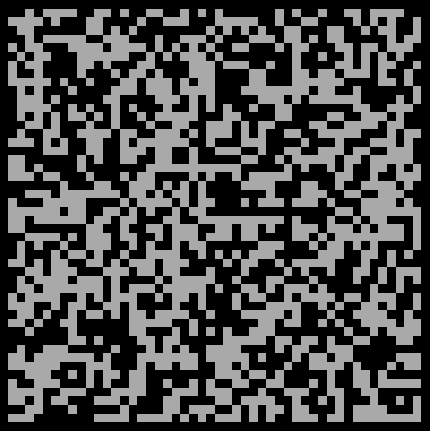
\includegraphics[width=\textwidth]{images/development/50_filled.png}
    \legend{Source: Image provided by author}
    \label{fig:fillper50}
  \end{minipage}
  \hfill
  \begin{minipage}[b]{0.4\textwidth}
    \caption{Map with fillPercent = 80.}
    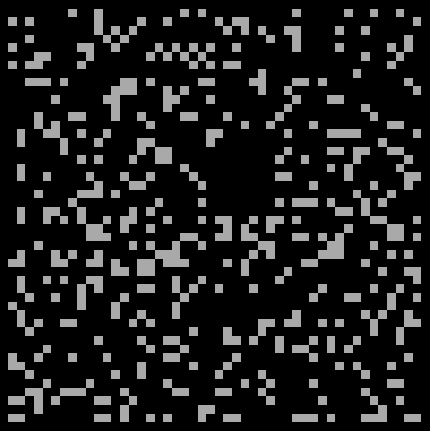
\includegraphics[width=\textwidth]{images/development/80_filled.png}
    \legend{Source: Image provided by author}
    \label{fig:fillper80}
  \end{minipage}
\end{figure}

The random number generator used can also be controlled by an user-defined parameter. The user can choose to write a \emph{seed} for the generator, in this case the generated map will always be the same for each given \emph{seed}. Otherwise, the \emph{seed} will be chosen automatically based on the execution time, making each generation different from the previous.

\section{Cellular automata}

A CA is a discrete model of computation first discovered by Stanislaw Ulam and John von Neumann; it can be described, in a simplified manner, as an \(n\)-dimmensional grid, a set of states and a set of transition rules. The grid is composed by cells, and these cells can be in one of several states; in the most basic form, cells can be 1 (on) or 0 (off) \cite{wolfram:1983}.

Although CA has found application in many different areas of study, it was the 1970s Conway's Game of Life which brought the it's attention to beyond academia. This was a zero person game where cells from a 2D grid would live or die (only two states, \(1\) or \(0\)) based on how many neighbors they had around them. This neighborhood is defined as the 8 cells surrounding the central cell currently being analyzed. Some of the rules from the Game of Life have been applied in dungeon generation, because of the cave-like appearance that the algorithm creates on the grid \cite{shaker:2016}.

In our specific case, the rule used is that, if there are more than \(4\) \emph{walls} around the current cell, then the cell becomes a \emph{wall}, if there are less then \(4\) \emph{walls} around the cell, it becomes a \emph{path}. The method was also chosen because it generates images that are similar to the representation of \emph{spongework} caves, shown in Figure \ref{fig:cave_patterns}. Figure \ref{fig:ca_rule} serves as a visual representation to this rule, where the red cell is the one being currently analyzed and the number on the right represents is resulting state after the CA pass.

\begin{figure}[h]
    \caption{Representation of the CA rule used.}
    \centerline{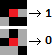
\includegraphics[width=4cm]{images/development/ca_rule.png}}
    \legend{Source: Image provided by author}
    \label{fig:ca_rule}
\end{figure}

In Figure \ref{fig:5itca} we can see the base map generated in Figure \ref{fig:fillper50} after \(5\) iterations of the CA. And Figure \ref{fig:20itca} shows the map after \(20\) iterations. The number of iterations is also a user-defined parameter for the system.

\begin{figure}[h]
  \centering
  \begin{minipage}[b]{0.4\textwidth}
    \caption{Map after 5 iterations of CA.}
    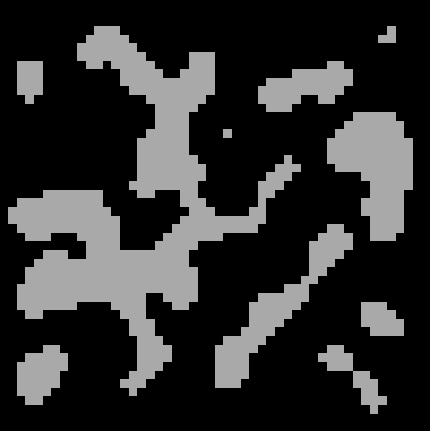
\includegraphics[width=\textwidth]{images/development/5it_ca.png}
    \legend{Source: Image provided by author}
    \label{fig:5itca}
  \end{minipage}
  \hfill
  \begin{minipage}[b]{0.4\textwidth}
    \caption{Map after 20 iterations of CA.}
    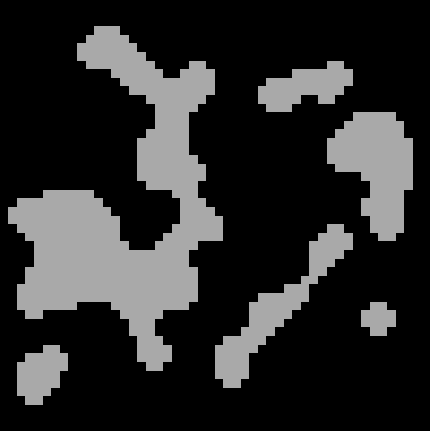
\includegraphics[width=\textwidth]{images/development/20it_ca.png}
    \legend{Source: Image provided by author}
    \label{fig:20itca}
  \end{minipage}
\end{figure}

\section{Create a list of rooms}

At this stage, we are left with one or more rooms scattered throughout the map. We can define room by one or more connected \emph{path} cells. On code, we represent the rooms as a separate \emph{Room} class, that contains the coordinates of all cells on the room. It's important to note that the \emph{Room} class also contains some other important information are used by the step that will be explained in Section \ref{sec:connection}: a flag saying if the \emph{Room} was visited, a list of \emph{Rooms} connected to this \emph{Room}, a method that connects two \emph{Rooms}.

There are two sets of user-defined inputs that will determine: if there will be entrance and exit rooms created; and their location on the map. After the creation of these rooms, we go through the map grid and search for paths, if a path was found we use the flood-fill algorithm in order to define where this room begins and ends, and then create a \emph{Room} containing all the coordinates of its cells. After the creation of the \emph{Room}, we add it to a list, containing all \emph{Rooms} on the map.

\section{Checking if the generated map is possible}
\label{sec:check_poss}

One of the issues that came up during development is that not all generated maps can translate well to a 2D top-down tile-based map. This happens because, for a visually well-formed wall to be generated, there needs to have at least \(2\) \emph{walls} between \(2\) \emph{paths}. Figure \ref{fig:malformed_wall} exemplifies a malformed wall between 2 \emph{Rooms}.

\begin{figure}[h]
    \caption{Example of a malformed wall between two \emph{Rooms}}
    \centerline{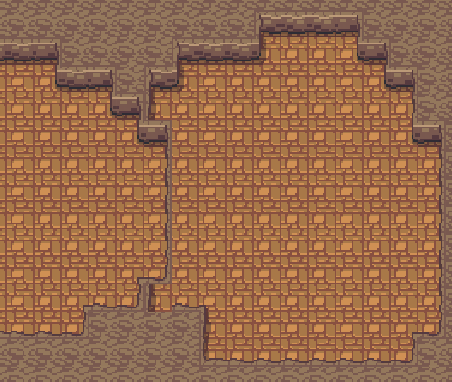
\includegraphics[width=10cm]{images/development/deformed_wall.png}}
    \legend{Source: Image provided by author}
    \label{fig:malformed_wall}
\end{figure}

In this step we go through each cell of each \emph{Room} and check if there are \emph{Rooms} that have a distance of less then \(2\) cells from each other. If there are, then the whole process is started again until the generated \emph{Room} can be translated well to a tile-based map. Algorithm \ref{alg:check_possible} describes this process.

\begin{algorithm}[h]
 \DontPrintSemicolon
 \While{map is not possible}{
  Randomly fill the map\;
  Run cellular automata\;
  Create a list of Rooms\;
  Check if the generated map is possible\;
 }
 \caption{Checking if the generated map is possible}
\label{alg:check_possible}
\end{algorithm} 

\section{Connection between rooms}
\label{sec:connection}

We will divide this section into 2 steps: ensuring connectivity through graph algorithms and drawing the connection using Bresenham's line algorithm.

\subsection{Ensuring connectivity}

Ensuring the connectivity between all rooms is important for a reason cited on Section \ref{sec:goodmap} of Chapter \ref{chapter:proposal}: "Dungeon maps should have an entrance, an exit (sometimes being the same), and a path between them". For our specific case, there is one more reason why this step is important: making maps that are similar to the \emph{branchwork} or \emph{network} cave patterns.

We need to make sure that every pair of \emph{Rooms} are connected, i.e., there is a way to reach one \emph{Room} by starting on the other \emph{Room}. All of \emph{Rooms} in the map can be viewed as nodes in a graph, that way, we made use of a popular algorithm in graph theory to check if there's connectivity: depth-first search.

Figure \ref{fig:connectivity} shows a visual representation of Algorithm  \ref{alg:connectivity} used in this step. The nodes of the graph represent \emph{Rooms} in the map. In quadrant \(1\) we start with a map with fully disconnected \emph{Rooms}. We begin by connecting each node to its closest node in quadrant \(2\); then we do a depth-first search to check if connectivity is ensured; if it's not, we treat the sets of connected nodes as one node like is shown on quadrant \(3\), and then redo the connection step, the result can be seen in quadrant \(4\).

\begin{figure}[h]
    \caption{Visual representation of the connectivity algorithm.}
    \centerline{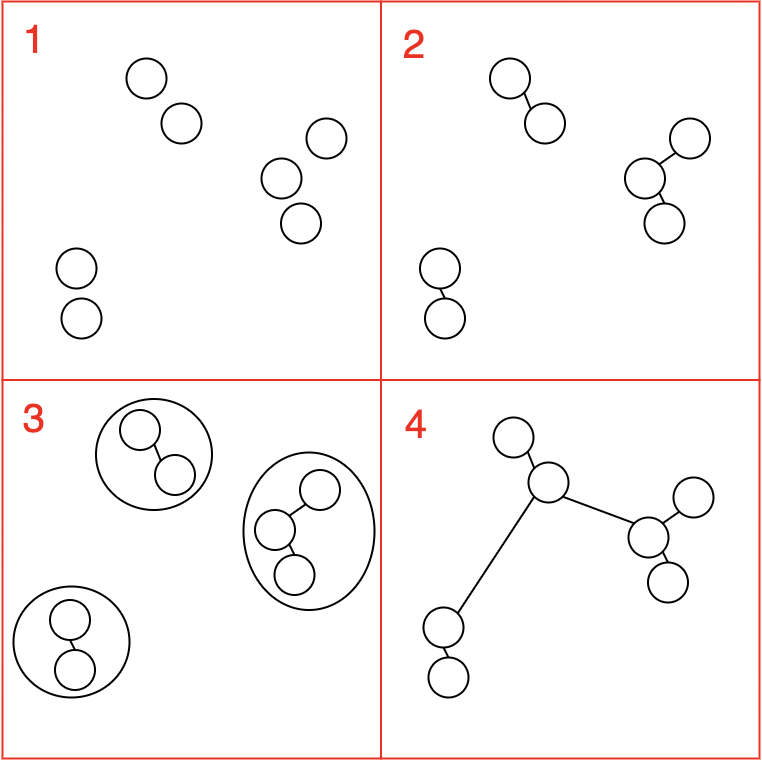
\includegraphics[width=7cm]{images/development/graph_connect.png}}
    \legend{Source: Image provided by author}
    \label{fig:connectivity}
\end{figure}

\begin{algorithm}[h]
 \DontPrintSemicolon
 Graph = represent Rooms as graph\;
 \While{connectivity isn't reached}{
  Connect closest Rooms in Graph\;
  Check connectivity\;
  Transform the sets of connected Rooms into new nodes for the new Graph\;
 }
 \caption{Ensuring connectivity of the map}
\label{alg:connectivity}
\end{algorithm} 

\subsection{Drawing the connection}

At this point we have a map filled with \emph{Rooms} that have ensured connectivity, but this connectivity is only represented by some elements of the \emph{Room} class, it is not yet represented in the map grid as \emph{walls} and \emph{paths}.

This is where the algorithm known as Bresenham's line is used. This algorithm, suggested in 1962 by Jack Elton Bresenham, is used to determine which points on an \(n\)-dimensional raster should be selected in order to form a close approximation of a straight line \cite{bresenham:1965}. 

Since each \emph{Room} has all of its cell coordinates stored, we can choose the closest cells for each connection and then use the Bresenham's line algorithm to draw this line on the map. Figure \ref{fig:map_connected} shows the same map from Figure \ref{fig:20itca} after the connectivity is ensured and then drawn on the map.

It may seem like these passages will not allow the player to pass through them, but the nature of the chosen tileset allows this passage to happen, as shown in Figure \ref{fig:it_works}.

\begin{figure}[h]
    \caption{Map after connectivity is ensured.}
    \centerline{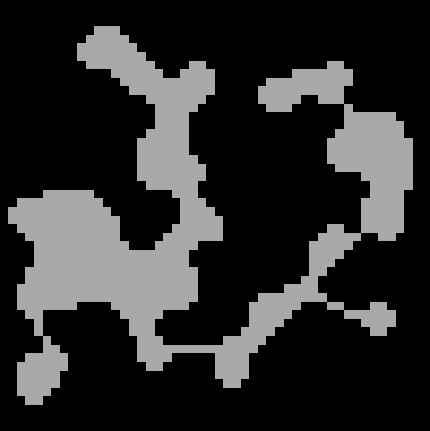
\includegraphics[width=7cm]{images/development/after_connection.png}}
    \legend{Source: Image provided by author}
    \label{fig:map_connected}
\end{figure}

\begin{figure}[h]
    \caption{Passage before and after tile placement.}
    \centerline{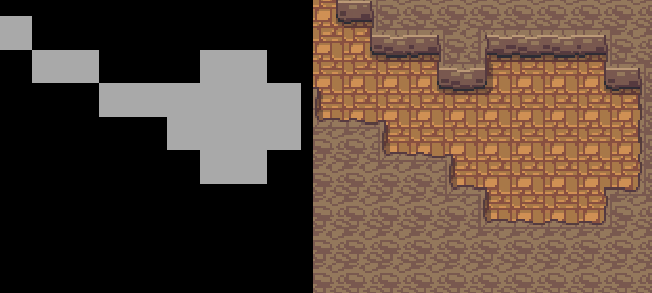
\includegraphics[width=7cm]{images/development/it_works.png}}
    \legend{Source: Image provided by author}
    \label{fig:it_works}
\end{figure}

\section{Remove inconsistencies from the map}

helo guys.

Just like in Section \ref{sec:check_poss}, maps that are generated with single-spaced \emph{wall} will not translate well to a 2D tile-map. Some of these problematic \emph{walls} sometimes are created on the process of drawing the Bresenham's lines connecting two \emph{Rooms}.

In this step we deal with these here called \emph{inconsistencies} by going through the entire map grid and checking for \emph{wall} cells that have either a \emph{path} to its right and left, here shown on Figure \ref{fig:hor_inc}; or to its up or down, as shown in Figure \ref{fig:ver_inc}; the inconsistencies are circled in red.

\begin{figure}[h]
  \centering
  \begin{minipage}[b]{0.4\textwidth}
    \caption{Example of a horizontal inconsistency.}
    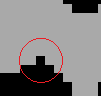
\includegraphics[width=\textwidth]{images/development/horizontal_incosistency.png}
    \legend{Source: Image provided by author}
    \label{fig:hor_inc}
  \end{minipage}
  \hfill
  \begin{minipage}[b]{0.4\textwidth}
    \caption{Example of a vertical inconsistency.}
    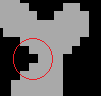
\includegraphics[width=\textwidth]{images/development/vertical_incosistency.png}
    \legend{Source: Image provided by author}
    \label{fig:ver_inc}
  \end{minipage}
\end{figure}

\section{Tile placement}

Finally, the last step of the generation is to place the tiles to their corresponding spots in the \emph{walls} and \emph{paths}.

There are a number of \(13\) \emph{wall} tiles needed to create the map, are shown here on Figure \ref{fig:wall_tiles}. There is only a single \emph{path} tile, which is visible on the resulted map in Figure \ref{fig:map_result}.

\begin{figure}[h]
    \caption{Wall tiles.}
    \centerline{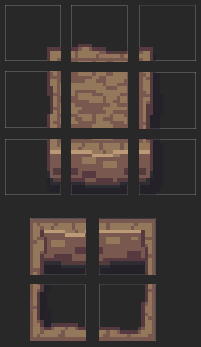
\includegraphics{images/development/wall_tiles.png}}
    \legend{Source: Image provided by author}
    \label{fig:wall_tiles}
\end{figure}

The first idea we had was to try to use a custom CA ruleset, where each cell had \(14\) possible states, one for each needed tile. But, since after only one passage of the ruleset through the map grid all the tiles were correctly placed, this algorithm can be better described as a morphological operation.

This ruleset, containing 14 rules, is here shown on Figure \ref{fig:ruleset}. The next item list serves to better understand the content of this Figure:

\begin{itemize}
    \item Similarly to Figure \ref{fig:ca_rule}, the center cell is the one currently being analyzed.
    \item Gray cells represent \emph{wall} cells.
    \item White cells represent \emph{path} cells.
    \item Pink cells represent either a \emph{wall} or a \emph{path}, meaning that the content of this cell doesn't matter, i.e., won't be analyzed by this rule.
    \item The tile after the rule number is what the rule will return for the cell being analyzed. 
\end{itemize}

For example, \emph{Rule 3} will check if the current cell is a \emph{wall}, then if the cell above the current is a \emph{path}, then if the cell to the left is a \emph{path}, then if the cell to the right is a \emph{wall}, then if the cell below is a \emph{wall} and finally if the cell to the bottom right is a \emph{wall}; if all of these conditions are met, the rule will return the corner tile shown on Figure \ref{fig:ruleset} for \emph{Rule 3} and place it on the analyzed cell.

\begin{figure}[h]
    \caption{Ruleset.}
    \centerline{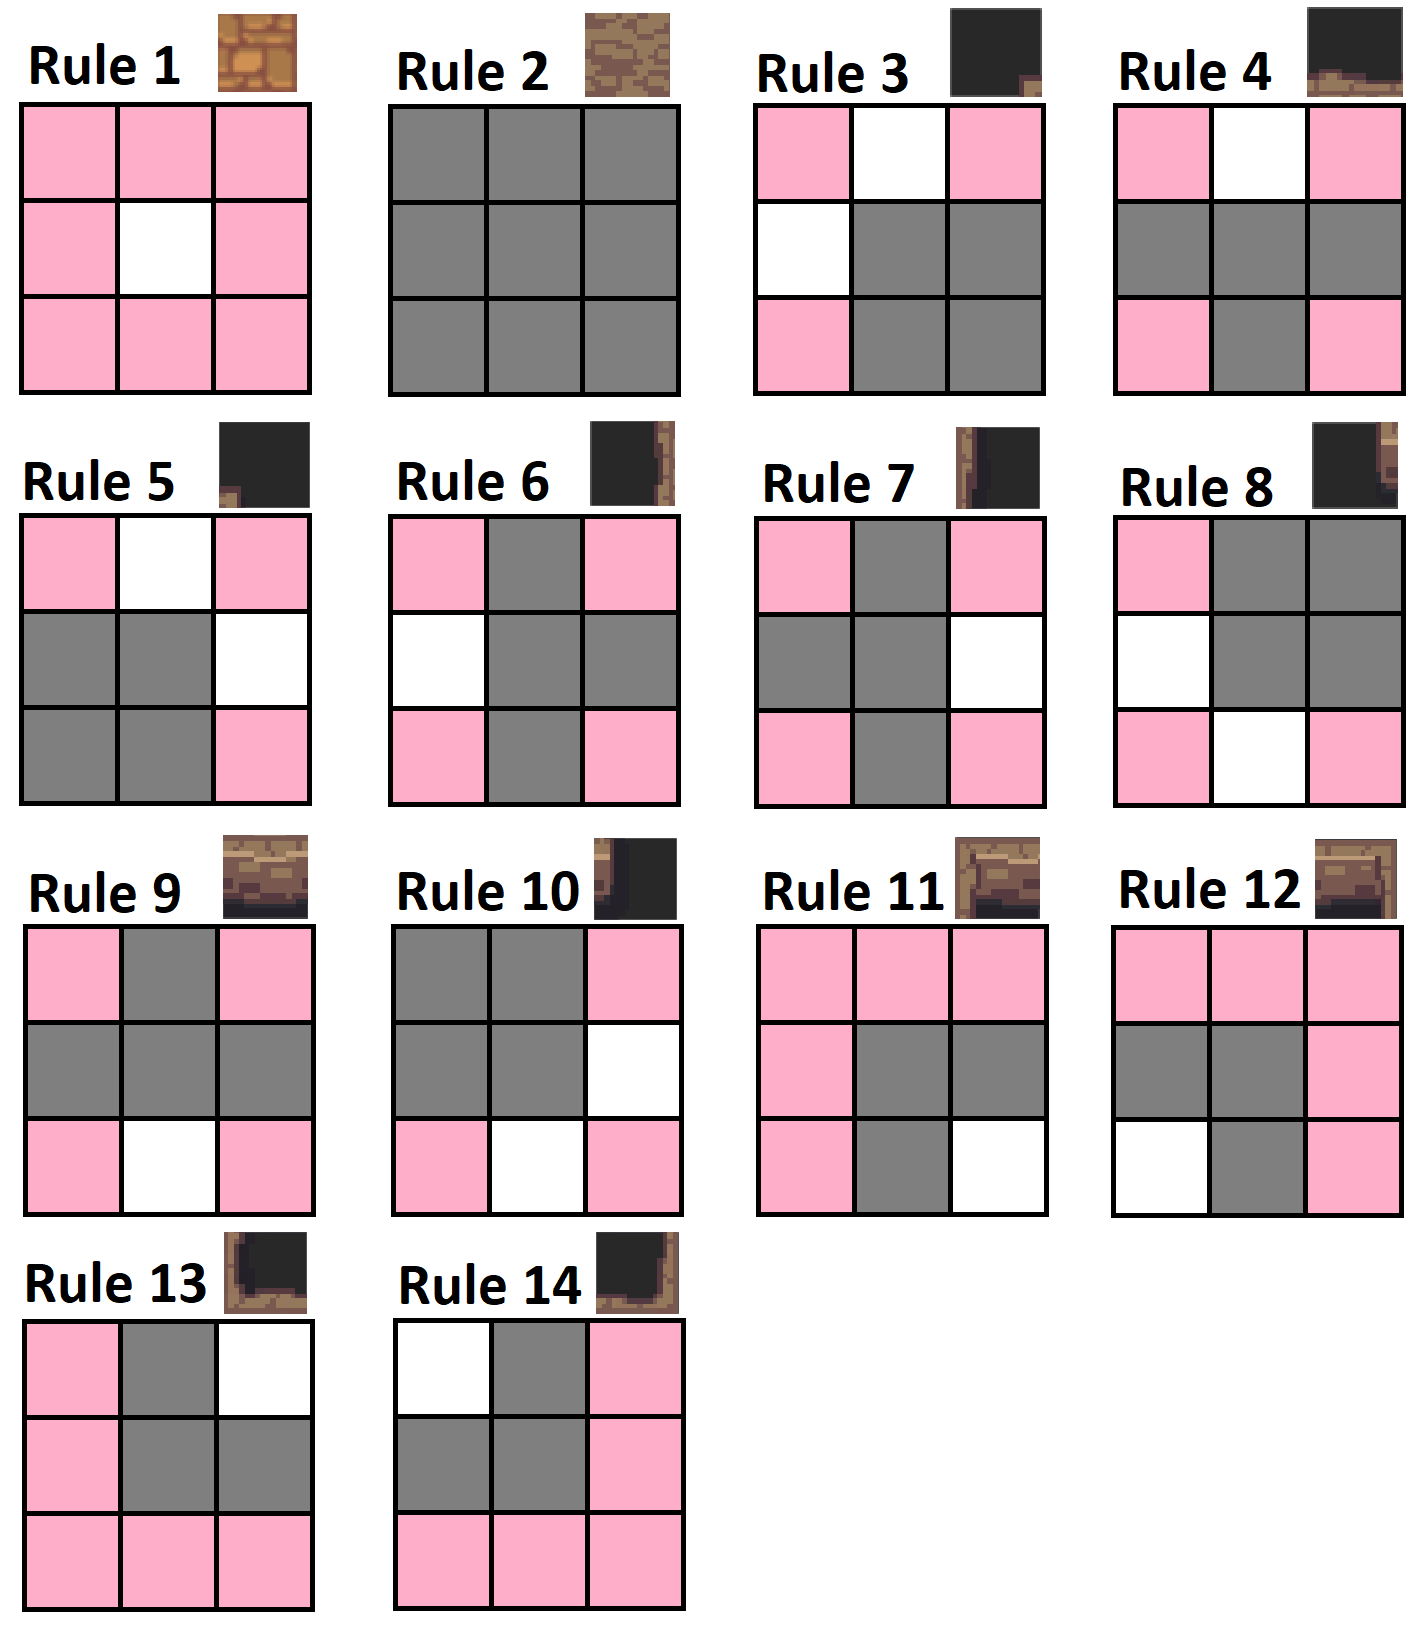
\includegraphics[width=12cm]{images/development/morph_rules.png}}
    \legend{Source: Image provided by author}
    \label{fig:ruleset}
\end{figure}

After the algorithm has gone through the whole map grid, the result will be a fully-formed 2D tile-based top-down map. Figure \ref{fig:map_result} shows the same map from Figure \ref{fig:map_connected} after the tile placement.

\begin{figure}[h]
    \caption{Resulting generated map.}
    \centerline{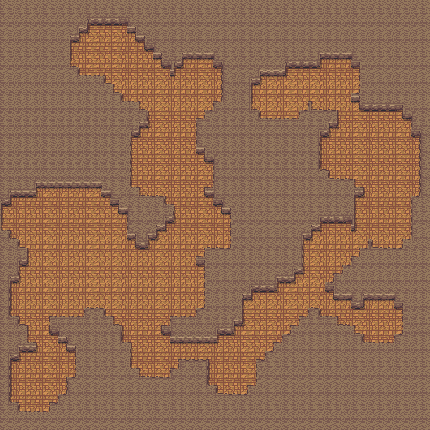
\includegraphics{images/development/final_result.png}}
    \legend{Source: Image provided by author}
    \label{fig:map_result}
\end{figure}

\section{User-defined parameters}

On this section we will be showcasing all of the user-defined parameters that can be used to tweak the generation of the map.

Figure \ref{fig:user_par} shows a snippet of the Unity tool, showing all the parameters used to generate the map shown on Figure \ref{fig:map_result}: \(w_{map} = h_{map} = 50\); the creation of a start and an end room was disabled; the number of iterations for the CA step was set to \(20\); a specific \emph{seed} was set; and the fill percent of the first step was set to \(50\). 

\begin{figure}[h]
    \caption{Available user parameters.}
    \centerline{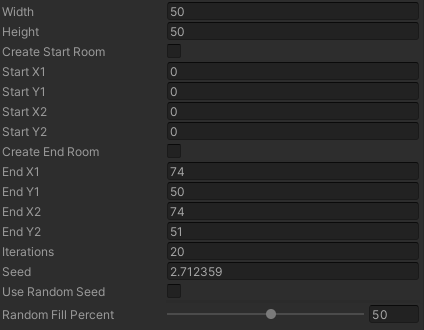
\includegraphics{images/development/user_parameters.png}}
    \legend{Source: Image provided by author}
    \label{fig:user_par}
\end{figure}